\chapter[Amplitude metrics for cellular bioluminescence reporters]{Amplitude metrics for cellular bioluminescence reporters\footnote{Portions of this chapter are published in P. C. St. John, S. R. Taylor, J. H. Abel, and F. J. Doyle, ``Amplitude Metrics for Cellular Circadian Bioluminescence Reporters,'' {\itshape Biophys. J.}, vol. 107, pp. 2712– 2722, Dec. 2014.}}
% \section{Motivation, link to previous chapter}\blindtext
% \subsection{Different enzymes control circadian rhythms at different phases}\blindtext
% \subsection{Perturbations likely have a time-dependent effect on amplitude}\blindtext
% \subsection{Comparison of Ukai vs Pulivarthy 2007}\blindtext
% \section{Single cell amplitude metrics}\blindtext
% \subsection{Definition of amplitude metric}\blindtext
% \subsection{Finite difference ARC}\blindtext
% \subsection{Derivation of sensitivity-based method}\blindtext
% \section{Population-level models}\blindtext
% \subsection{Definitions and diffusion-convection equation}\blindtext
% \subsection{Circular statistics}\blindtext
% \subsection{Inverting $p(\theta, \hat{t})$}\blindtext
% \subsection{Calculating $\bar{x}(\hat{t})$ and $\hat{x}(\hat{t})$}\blindtext

\section{Background}

In the previous chapter, I described used mathematical modeling to explain the systems-level effects of two pharmacological agents. 
In doing so, it was shown that each compound controlled reactions which primarily occur during specific times of day. 
Since clinical applications of circadian therapies will likely have a time at which they are administered, it is important to understand the effects of temporary perturbations on circadian amplitude. 
The effects of temporary perturbations are more complicated, however, since they may effect both the single-cell oscillator as well as the synchrony of cell populations as a whole.
In this chapter, I develop the mathematical background required to understand and efficiently predict the response of a population of oscillators to a temporary change.

\subsection{Importance of circadian amplitude}
% In mammals, circadian rhythms are endogenous oscillations in gene transcription responsible for coordinating daily changes in physiology.
While the suprachiasmatic nucleus (SCN) in the brain serves as the body's master pacemaker, cells found in peripheral tissues also oscillate in a circadian manner \cite{Lamia2008}.
These peripheral clocks process systemic and SCN-mediated entraining cues, buffering against rhythmic changes in energy availability to maintain metabolic homeostasis \cite{Kornmann2007}.
The amplitude of circadian transcription is a relevant factor, and has been shown to play a critical role in phase resetting and entrainment \cite{Pittendrigh1991, Abraham2010}.
Recent studies have further highlighted the importance of high peripheral clock amplitudes in maintaining metabolic health.
Mice lacking an intact clock have been shown to develop metabolic disease \cite{Marcheva2010}, while low amplitude clock oscillations, whether caused by diet \cite{Hatori2012} or age \cite{Chang2013} have also been tied to metabolic disorders.
An understanding of how clock amplitudes are regulated is therefore a topic of ongoing research with potential therapeutic applications \cite{St.John2014}.
Unlike the network of oscillators in the SCN, in which intercellular coupling maintains robust amplitudes even in the absence of external cues, peripheral oscillators are thought to lack a direct mechanism to spontaneously synchronize \cite{Welsh2004}.
As a result, populations of peripheral clocks are likely synchronized by common external cues, with stochastic effects and cell heterogeneity driving entrained populations gradually toward desynchrony.

\subsection{Amplitude at the single-cell and population level}
The development of immortalized peripheral oscillator cell lines with bioluminescent reporters has allowed high-throughput analysis of the responses of circadian rhythms to genetic and pharmacological manipulation \cite{Hirota2010, Ramanathan2014}.
In addition to providing experimental tractability, these systems provide detailed information on the amplitude of oscillations in gene transcription, a measure often lacking from earlier experiments using wheel-running activity.
 As a result, these cell lines have proven useful in studying core clock connectivity and stoichiometry \cite{Baggs2009}.
However, since {\itshape in vitro} experiments typically measure entire cultures of cells, data collected at the population-level can obscure the response of the clock at the scale of the gene-regulatory network.
Even when individual cells can be recorded, stochastic noise hinders accurate amplitude determination.
As a result, two studies using similar perturbations to understand the mechanism of light-induced amplitude reduction reached differing conclusions, in which either single-cell amplitude reduction or population-level desynchrony was identified as the dominant factor \cite{Pulivarthy2007, Ukai2007}.

\subsection{Role of mathematical modeling}
Mathematical models have long been used to understand the results of circadian experiments \cite{Leloup2003, Becker-Weimann2004}, aided by definitions and computational techniques designed to match modeling predictions to experimental data.
One such definition is the response function, a general technique that maps a change in an output variable to a temporary change in parameters \cite{Rand2004}.
For instance, the phase response curve (PRC) has been used to characterize the entrainment behavior of both experimental and mathematical systems \cite{Daan1976, Taylor2008, Pfeuty2011}, and in analyzing the synchrony of populations of oscillators \cite{Kim2014}.
Accurate and efficient numerical routines for finding infinitesimal PRCs have therefore been developed \cite{Kramer1984, Gunawan2006, Taylor2008a}.
In addition to changes in phase, phase-dependent changes in amplitude are an important factor in understanding circadian rhythms.
Amplitude response curves (ARCs) were first used in the clock literature to understand the effects of light pulses on simple phase-amplitude models, and were useful in predicting phase singularity behavior \cite{Jewett1998}.
ARCs have also been used to characterize perturbations to groups of oscillators through desynchrony \cite{Achermann1999, Ukai2007}, at the level of the single oscillator \cite{VanderVeen2012, Castejon2013}, and even in studying the effect of entrainment phase on SCN rhythm amplitude \cite{VanOosterhout2012}.
However, previous definitions of the ARC are inconsistent between studies and do not simultaneously consider amplitude effects at the single-cell and population level.

The choice of modeling framework dictates the type of amplitude response which can be predicted.
Ordinary differential equation (ODE) models of gene regulation are capable of describing the amplitude and phase-resetting behavior of single cells, but fail to capture the collective dynamics of a population of oscillators.
Likewise, phase-only models correctly capture the change in synchrony of a population, but do not capture fluctuations in amplitude of individual oscillators.
Explicit stochastic simulations of populations of cells are capable of realistically capturing both single-cell and population-level effects, and have been successfully used to understand the response of coupled oscillators to external VIP perturbation \cite{An2013}.
However, these methods are computationally expensive, and cannot be used for an analytical understanding of amplitude response.

In this chapter, I describe approaches to quantify amplitude change in a population of non-interacting oscillators.
By exploiting the independence of each oscillator, we derive computationally efficient methods to approximate the mean dynamics of full stochastic simulations.
Additionally, our method allows the calculation of ARCs at both the single-cell and population level, allowing the behavior of the system to be quickly profiled.
Specifically, we use ODE models to describe the transient amplitude response at the single-cell level, coupled with a phase probability density function to describe population-level dynamics.
Following a perturbation with a finite duration, a limit cycle oscillator undergoes a transient change in amplitude.
When the mean expression level of a population of oscillators is also considered, an additional change in amplitude is incurred due to the change in synchrony of the population, which persists until synchrony is changed by subsequent perturbations.
We therefore observe a separation in timescales between the effects on clock output mediated at the single-cell level and those mediated by population synchrony, allowing the source of an amplitude change to be qualitatively inferred by inspection of bioluminescence data.
Characterizing the mechanisms and consequences of both types of amplitude regulation will be important in understanding how peripheral amplitudes are maintained, and may lead to the design of pharmacological or behavioral strategies to boost circadian amplitudes.


\section{Materials and Methods}

% Move most of these to the introduction?
\subsection{Basic definitions}

Ordinary differential equation (ODE) models take the general form
\begin{equation}
  \frac{dx}{dt} = f(x(t), p),
  \label{eq:odefn}
\end{equation}
in which $x(t)$ represents the concentrations of the state variables, such as mRNA and protein concentrations, $f$ contains information on the production, degradation, and reactivity of the states, and $p$ are the kinetic parameters which govern reaction kinetics.
Limit cycle models are ODE models in which the solution approaches a steady state oscillatory trajectory, satisfying the equation:
\begin{equation}
  \lim_{t \to \infty} \left[ x(t + T) - x(t) \right] = 0.
  \label{eq:limit5}
\end{equation}
The period is the smallest $T > 0$ for which \fref{eq:limit5} holds.
The points on the stable limit cycle are denoted by $x^\gamma(\theta)$ with each point assigned to a value of a phase variable $\theta \in [0, 2\pi)$.
For convenience, time in \fref{eq:odefn} can be rescaled such that the period is $2\pi$:
\begin{equation}
  \tilde{t} = \frac{2\pi}{T}t; \quad \tilde{f} = \frac{T}{2\pi}\;f; \quad \frac{dx}{d\tilde{t}} = \tilde{f}(x(\tilde{t}), p).
  \label{eq:that}
\end{equation}
The phase variable $\theta$ is therefore defined on the limit cycle as $\theta = \tilde{t}\mod 2\pi$, with $\theta = 0$ assigned to a unique and identifiable point.

\subsection{Perturbations to limit cycle systems}

In this chapter we restrict our analysis to temporary perturbations capable of entraining an oscillatory system, excluding permanent parameter changes arising, for instance, from genetic knockout experiments.
The most simple entraining perturbation involves adding or removing components to a limit cycle system, resulting in a perturbed trajectory $x(t)$.
Here the initial conditions are determined by the strength of the perturbation and the phase at which it is applied:
\begin{equation}
  x(0) \coloneqq x^\gamma(\theta_0) + \Delta x(0).
  \label{eq:stateperturbation}
\end{equation}
This trajectory evolves according to \fref{eq:odefn}, eventually returning to $x^\gamma$.
It is useful to express this trajectory by the deviation from the limit cycle:
\begin{equation}
  \Delta x(\tilde{t}) = x(\tilde{t}) - x^\gamma(\tilde{t} + \theta_0).
  \label{eq:delxt}
\end{equation}

In addition to perturbations directly to the state of the system, oscillators can also be perturbed by temporary changes to the parameters.
For a parameter pulse $\Delta p$ of duration $\tilde{d}$ (in radians) that ends at $\theta_0$, the oscillator deviates from the limit cycle trajectory according to:
\begin{align}
  x_{\tilde{d}}(-\tilde{d}) &= x^\gamma(\theta_0 - \tilde{d}) \\
  \frac{dx_{\tilde{d}}}{d\tilde{t}} &= \tilde{f}(x_{\tilde{d}}(\tilde{t}), p + \Delta p) \label{eq:ode_pert}.
\end{align}
The pulse trajectory $x_{\tilde{d}}(\tilde{t})$ is then integrated from $\tilde{t} = -\tilde{d} \to 0$, at which point the pulse is removed.
A temporary parameter pulse is therefore equivalent to a state perturbation, but with the perturbation at $t = 0$ defined by:
\begin{equation}
  \Delta x(0) = x_{\tilde{d}}(0) - x^\gamma(\theta_0).
\end{equation}
A schematic depicting an example perturbed and reference trajectory is shown in \fref{fig:51schem}.

\begin{figure}[tbp]
  \begin{center}
    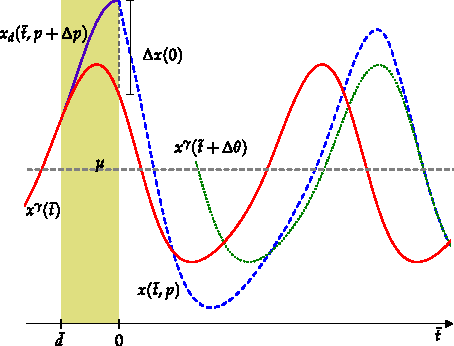
\includegraphics[width=.75\textwidth]{chap5/figures/figure_1_schem.pdf}
  \end{center}
  \titlecaption{Schematic showing trajectories used in the calculation of single-cell phase and amplitude change}{A perturbation $x(\tilde{t},p)$, blue, from the limit cycle solution $x^\gamma(\tilde{t},p)$, red, ultimately returns to the limit cycle with a phase shift $x^\gamma(\tilde{t} + \Delta\theta,p)$, green.}
  \label{fig:51schem}
\end{figure}

The response of the system to very small perturbations is more efficiently calculated using ODE sensitivity analysis \cite{Rabitz1983}.
The sensitivity matrix,
\begin{equation}
  S(t) = \frac{dx(t)}{dx(0)} = \lim_{\Delta x(0) \to 0}\frac{\Delta x(t)}{\Delta x(0)},
  \label{eq:senslimit}
\end{equation}
can be calculated directly by integrating
\begin{equation}
  \frac{d}{dt} S(t)  = \frac{df(x(t),p)}{dx}\; S(t)
  \label{eq:odesens}
\end{equation}
with $S(0) = I$.

\subsection{Phase response curves}
Quantifying phase changes following a perturbation has been well studied and is particularly relevant for models of circadian rhythms \cite{Kramer1984, Taylor2008a}.
A phase response curve (PRC) maps the change in phase resulting from the same perturbation applied at each initial phase.
Infinitesimal PRCs, the derivative of the phase change with respect to the perturbation, can be defined for state and parameter-impulse perturbations \cite{Taylor2008a}.
Methods for efficiently calculating these quantities using ODE sensitivity analysis have been developed \cite{Taylor2008a}, with the important result that the parameter- and state-impulse PRCs can be related by the Jacobian matrix:
\begin{equation}
  \frac{d}{d\tilde{t}}\frac{d\theta}{dp} = \frac{d\theta}{dx}\frac{d\tilde{f}}{dp}.
  \label{eq:pPRCequiv}
\end{equation}
This result follows from the fact that in the limit of an infinitely short and small parameter pulse, $\Delta x(0) \to \nicefrac{d\tilde{f}}{dp}\,\tilde{d}\, \Delta p$.

\subsection{Phase-diffusion model}
Large populations of oscillators are typically described using phase-only models \cite{Rougemont2006}, in which the state of each oscillator is represented only by its phase, $\theta$.
The synchrony of the population can be modeled using a probability density function $p(\theta, \tilde{t})$ that describes the probability of finding an oscillator at each phase \cite{Kuramoto1984}.
The usefulness of probability density functions in describing the phase and amplitude responses of populations of circadian cells has been previously shown \cite{Ukai2007}.
As with all probability density functions,
\begin{equation}
  \int_0^{2\pi} p(\theta, \tilde{t}) \; d\theta = 1.
\end{equation}
The shape of $p(\theta, \tilde{t})$ changes as the cells advance in time.
Stochastic effects cause the population to gradually desynchronize as slight cycle-to-cycle deviations are propagated throughout the population \cite{Teramae2004}.
For a infinite population of oscillators, these effects are well-described by a Fokker-Plank equation \cite{Stein1965}:
\begin{equation}
  \frac{\partial p}{\partial \tilde{t}} = \frac{\partial p}{\partial \theta} + d\frac{\partial^2 p}{\partial \theta^2}.
  \label{eq:pde}
\end{equation}
Due to the rescaling of $t$, the mean period of the population is $2\pi$.
Here, the $\nicefrac{\partial p}{\partial \theta}$ term, analogous to convection, describes the mean oscillatory period, while the $\nicefrac{\partial^2 p}{\partial \theta^2}$ term describes the diffusion of phases across $[0, 2\pi)$.
The phase diffusivity parameter $d$ (in units of inverse radians) describes the speed with which the population desynchronizes and can be fit to experimental data \cite{Rougemont2007}.
\fref{eq:pde} has periodic boundary conditions, with initial condition $\phi(\theta)$ as the phase population at $t=0$:
\begin{align}
  \text{BCs:}\quad p(0, \tilde{t}) &= p(2\pi, \tilde{t}) \\
  \frac{\partial p}{\partial \theta}(0, \tilde{t}) &= \frac{\partial p}{\partial \theta}(2\pi, \tilde{t}) \\
  \text{IC:}\quad p(\theta, 0) &= \phi(\theta).
  \label{eq:pde_ic}
\end{align}
The solution of equations~(\ref{eq:pde}-\ref{eq:pde_ic}) is well-characterized, with $p(\theta, \tilde{t})$ evolving in time as the convolution of the initial conditions with a wrapped normal distribution with mean $\tilde{t}$ and standard deviation $\sqrt{2d\tilde{t}}$ \cite{Chirikjian2009}:
\begin{equation}
  p(\theta, \tilde{t}) = \phi(\theta) * \mathcal{WN}(\theta; \tilde{t},
  \sqrt{2\, d\, \tilde{t}}),
\end{equation}
in which the wrapped normal distribution \cite{Mardia2009} is defined as
\begin{equation}
  {\cal WN}(\theta; \mu, \sigma) =
  \frac{1}{\sigma\sqrt{2\pi}}\sum_{k=-\infty}^\infty \exp\left[\frac{-(\theta
  - \mu + 2\pi k)^2}{2\sigma^2}\right].
  \label{eq:wrapped_normal}
\end{equation}
Since the convolution of two normal distributions is also a normal distribution, it is efficient when possible to describe $\phi(\theta)$ as a normal distribution with mean $\mu_0$ and standard deviation $\sigma_0$, such that $p(\theta, \tilde{t})$ can be found analytically through
\begin{equation}
  p(\theta, \tilde{t}) = \mathcal{WN}(\theta; \mu_0 + \tilde{t},
  \sqrt{\sigma_0^2 + 2d^2\tilde{t}^2}).
\end{equation}

\subsection{Numerical simulations}

ODE models were simulated in Python, using the computer algebra package CasADi \cite{Andersson2013b}.
Stochastic simulations were performed using the StochKit2 package \cite{Sanft2011a}.
The codes used to generate the figures are included as a supplemental file.

\section{Results and Discussion}

A signal to a population of limit cycle oscillators can affect amplitude in two ways.
First, individual cells are perturbed from their limit cycles, and exhibit transient dynamics before settling back to steady state amplitudes.
Secondly, the phases of the population are changed, resulting in a permanent change in population synchrony.
Therefore, in order to derive continuous approximations to the dynamics of a large population of non-interacting oscillators, we first demonstrate how ARCs can be found at both the single-cell and population level.

\subsection{Definition of an amplitude metric at the single-cell level}

Following a perturbation to a single cell, the path that the perturbed trajectory $x(t)$ takes in returning to the limit cycle will have a different amplitude than the unperturbed trajectory.
While such an amplitude change will only have a finite duration, it plays an important role when perturbations are repeatedly received by the clock, such as a peripheral oscillator entrained to daily metabolic stimuli.
To define an amplitude change metric for such a case, we compare a perturbed trajectory $x(t)$ to a phase-shifted limit cycle reference $y(t)$, for which $x(t) \to y(t)$ for sufficiently long times.
Since $x(t)$ approaches the reference as $t \to \infty$, the means of both trajectories are equal and can be calculated by
\begin{equation}
  \mu \coloneqq \int_0^{2\pi} \frac{x^\gamma(\theta)}{2\pi} \; d\theta.
  \label{eq:mu}
\end{equation}
The amplitude change metric is defined as
\begin{equation}
  \begin{aligned}
    \Delta A (x(t), y(t)) &\coloneqq \int_0^\infty (x(t) - \mu)^2 - (y(t) - \mu)^2 \; dt\\
    &= \int_0^\infty h(t) \; dt.
  \end{aligned}
  \label{eq:ampchangedefinition}
\end{equation}
This amplitude metric was chosen over alternatives, such as peak-trough distance, for its analytical tractability.
The integrand in \fref{eq:ampchangedefinition}, abbreviated by $h(t)$, compares the variances of the reference and perturbed trajectories.
When $h(t) > 0$, the trajectory is further from the mean than the reference, and similarly when $h(t) < 0$ the trajectory is closer to the mean than the reference.
Thus the overall amplitude change can be calculated by integrating $h(t)$ until the two trajectories converge, returning an amplitude value for each state variable.
Amplitude change for a two-dimensional oscillator is easy to visualize graphically.
In \fref{fig:51b}, the same state perturbation $\Delta x(0)$ applied at two different phases results in opposite amplitude changes, depending on whether the perturbation shifts the trajectory to the interior of the limit cycle (reduced amplitudes) or to the outside the limit cycle (increased amplitudes).
Trajectories for the second state variable, $Y(\tilde{t})$, and the corresponding integrand for the amplitude change equation, $h(\tilde{t})$, demonstrate how this transient change is quantified.

\begin{figure}[tbp]
  \begin{center}
    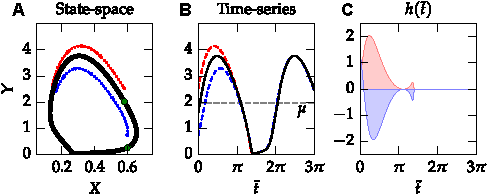
\includegraphics[width=.75\textwidth]{chap5/figures/figure_1_b.pdf}
  \end{center}
  \titlecaption{Amplitude metrics at the single-cell level measure transient deviations from the limit cycle}{The same perturbation applied at two different phases can result in opposite amplitude effects. The state-space representation ({\bfseries B}) reveals the path both perturbations take to return to the limit cycle. The time-series representation ({\bfseries C}) shows how the perturbation in blue results in an amplitude decrease, while the one in red results in an amplitude increase. ({\bfseries D}) This amplitude change is quantified by integrating $h(\tilde{t})$, the difference in variance from each solution to the limit cycle as defined in \fref{eq:ampchangedefinition}, from $t=0 \to \infty$. Here the shaded region indicates the area under the curve, $\Delta A$, for the perturbations shown in red and blue. Model adapted from \cite{Novak2008}.}
  \label{fig:51b}
\end{figure}

\subsection{Single-cell amplitude response curves}
Similar to the PRC, we denote the phase-dependent amplitude change following a perturbation as an amplitude response curve (ARC), using the metric presented in \fref{eq:ampchangedefinition}.
In \fref{fig:52}, we calculate the PRC and ARC for a state perturbation of three different strengths.
The weakest perturbation results in type 1 (weak) resetting, in which the phase response curve is continuous, while the strongest perturbation results in type 0 (strong) resetting, in which the PRC is discontinuous.
This transition occurs once the state perturbation is strong enough to push the trajectory over the unstable fixed point located at the middle of the limit cycle.
For a perturbation of intermediate strength, at a critical phase the trajectory will be pushed close to the fixed point and take a long time to recover the steady state amplitude.
The behavior at this singularity point is indicated by a sharp dip in the ARC for this perturbation strength.

\begin{figure}[tbp]
  \centering
  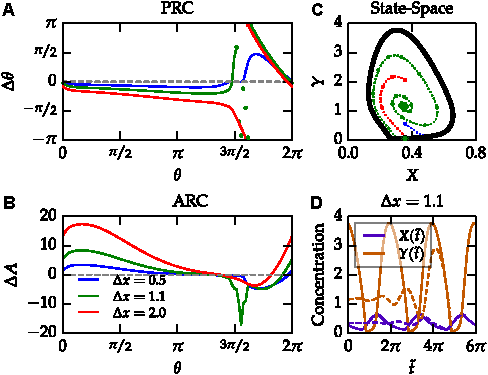
\includegraphics[width=.75\textwidth]{chap5/figures/figure_2.pdf}
  \titlecaption{Phase and amplitude response curves describe how a single oscillator will respond to a perturbation}{({\bfseries A-B}) The phase and amplitude response curves for three perturbations of increasing strengths demonstrate the transition from type 1 phase resetting for a weak stimulus (blue) to type 0 phase resetting from a strong stimulus (red). ({\bfseries C}) The state space representation for the perturbations of varying strengths demonstrate how the trajectories return to the limit cycle. For the particular perturbation shown in green, the trajectory starts very close to the singularity, and therefore takes a long time to recover. ({\bfseries D}) For an oscillator perturbed to the singularity, a strong amplitude reduction ensues. Here, the oscillator with an initial phase $\theta \approx \nicefrac{3\pi}{2}$ is perturbed by $\Delta x = 1.1$ at $\tilde{t} = 0$. Several cycles are required for normal amplitudes to be restored, corresponding to a dip in the ARC (C, green).}
  \label{fig:52}
\end{figure}

Infinitesimal versions of response curves are often more general and easier to compute than those that track a specific perturbation strength \cite{Rand2004}.
We therefore derive an expression for the infinitesimal ARC, defined as
\begin{equation}
  \frac{dA}{dx} \coloneqq \lim_{\Delta x(0) \to 0} \frac{\Delta A\left(x(\tilde{t}),\ x^\gamma(\tilde{t} + \theta_0 + \Delta\theta)\right)}{\Delta x(0)} = \int_0^\infty \lim_{\Delta x(0) \to 0} \frac{h(t)}{\Delta x(0)} \; dt.
  \label{eq:sARC}
\end{equation}
While this quantity could be calculating by using a very small $\Delta x(0)$, it is more accurate and efficient to derive a direct method to calculate \fref{eq:sARC} using the ODE sensitivities defined in \fref{eq:odesens}.
For simplicity, we define $t_\theta = \tilde{t} + \theta_0$, which allows the time variable for the perturbation to vary from $0 \to \infty$ while tracking the appropriate phase on the limit cycle.
Since $\Delta \theta \to 0$ as $\Delta x(0) \to 0$, we Taylor expand the limit cycle trajectory around $t_\theta$:
\begin{align}
  x^\gamma(t_\theta + \Delta\theta) &= x^\gamma(t_\theta) +
  \frac{dx^\gamma(t_\theta)}{d\theta}\Delta\theta + O(\Delta\theta^2)\\
  &= x^\gamma(t_\theta) + \tilde{f}\left(x^\gamma(t_\theta)\right)\Delta\theta +
  O(\Delta\theta^2).
\end{align}
Simplifying the integrand in \fref{eq:sARC},
\begin{align}
  \frac{h(t)}{\Delta x(0)} &= \frac{1}{\Delta x(0)} \left[\left(x^\gamma(t_\theta) + \Delta x(\tilde{t}) - \mu\right)^2 - \left(x^\gamma(t_\theta + \Delta \theta) - \mu\right)^2 \right]\\
  &= \frac{1}{\Delta x(0)} \left[\left(x^\gamma(t_\theta) + \Delta x(\tilde{t}) - \mu\right)^2 - \left(x^\gamma(t_\theta) + \tilde{f}\left(x^\gamma(t_\theta)\right)\Delta\theta - \mu\right)^2 \right]\\
  &= \frac{1}{\Delta x(0)} \left[\left(\Delta x(\tilde{t}) - \tilde{f}\left(x^\gamma(t_\theta)\right)\Delta\theta\right) \left(\Delta x(\tilde{t}) + \tilde{f}\left(x^\gamma(t_\theta)\right)\Delta\theta + 2(x^\gamma(t_\theta) - \mu)\right) \right].
\end{align}
Taking the limit of this integrand as $\Delta x(0) \to 0$ cancels several differential terms, and allows the remainder to be substituted with quantities that can be calculated using ODE sensitivity analysis:
\begin{align}
  \lim_{\Delta x(0) \to 0} \frac{h(t)}{\Delta x(0)} &= 2\left(\lim_{\Delta x(0) \to 0}\frac{\Delta x(\tilde{t})}{\Delta x(0)} - \tilde{f}\left(x^\gamma(t_\theta)\right)\lim_{\Delta x(0) \to 0}\frac{\Delta\theta}{\Delta x(0)}\right) \left(x^\gamma(t_\theta) - \mu\right)\\
  &= 2\left(S(\tilde{t}) - \tilde{f}(x^\gamma(t_\theta))\frac{d\theta}{dx}\right)\left(x^\gamma(t_\theta) - \mu\right).
  \label{eq:sens_sub}
\end{align}
Note that in \fref{eq:sens_sub}, $\nicefrac{d\theta}{dx}$ represents the derivative of $\Delta\theta$ with respect to the perturbation, and is therefore a scalar quantity.
The infinitesimal state-impulse ARC may therefore be calculated directly from the ODE sensitivity matrix and the PRC, allowing the amplitude change for an infinitesimal perturbation to be calculated exactly and efficiently:
\begin{equation}
  \frac{dA}{dx} = \int_0^\infty 2\left(S(\tilde{t}) - \tilde{f}(x^\gamma(t_\theta))\frac{d\theta}{dx}\right)\left(x^\gamma(t_\theta) - \mu\right) \; dt.
  \label{eq:siARC}
\end{equation}
Here, the first term of the integrand $(S - \tilde{f}\dot{\theta})$ tracks the distance from the perturbed trajectory to the limit cycle, which decays to zero as $t \to \infty$.
The second term $(x^\gamma - \mu)$ weights this distance by whether or not the deviation occurs above or below the oscillatory mean, yielding negative amplitude changes when the trajectory is perturbed closer to the mean.
Just as with the parameter-impulse PRC, the infinitesimal parameter-impulse ARC is defined as
\begin{equation}
  \frac{d}{d\tilde{t}}\frac{dA}{dp} \coloneqq \lim_{\tilde{d},\; \Delta p \to 0} \frac{\Delta A}{\tilde{d}\, \Delta p},
\end{equation}
and may be calculated from the state-impulse version with the following relationship:
\begin{equation}
  \frac{d}{d\tilde{t}}\frac{dA}{dp} = \frac{dA}{dx}\frac{d\tilde{f}}{dp}.
    \label{eq:piARC}
\end{equation}
As with \fref{eq:pPRCequiv}, this equivalency reflects the fact that for a pulse of infinitely short duration, a parameter change is equivalent to changing the state of the system along the direction specified by the Jacobian.
Convergence between the methods in equations~(\ref{eq:siARC}-\ref{eq:piARC}) and finite-difference approaches is shown in \fref{fig:5s1}, which demonstrates that the numerically-efficient differential ARCs remain representative even for moderate-strength perturbations.

\begin{figure}[tbp]
  \centering
  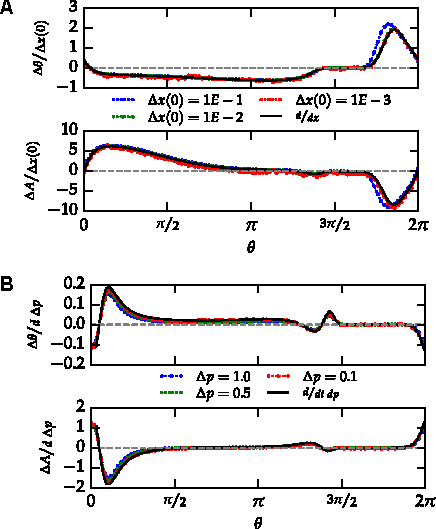
\includegraphics[width=.75\textwidth]{chap5/figures/figure_S1.pdf}
  \titlecaption{Convergence of finite-difference and differential methods}{({\bfseries A}) Perturbations of decreasing strength to the state of the oscillator result in phase and amplitude response curves that match the differential limit. ({\bfseries B}) Temporary perturbations of decreasing strength to a kinetic parameter. The duration of each perturbation is fixed to 0.2 radians. Finite difference approximations closely match the differential method, which is offset in phase by 0.1 radians to account for the nonzero pulse duration.}
  \label{fig:5s1}
\end{figure}


\subsection{Population-level response curves}

We next briefly describe how to calculate the PRC and ARC for a phase-density model.
These approaches are commonly used in understanding phase models \cite{Kuramoto1984, Ukai2007}, and are presented here to match previous definitions for single cells.
A phase transition curve, $g(\theta) = \theta + \Delta\theta$, maps the phase of an oscillator before perturbation to its phase after the perturbation.
Since individual oscillators are neither created nor destroyed during the perturbation, it is possible - yet numerically difficult - to directly calculate the phase probability distribution following perturbation using the standard change of variables relation:
\begin{equation}
  \hat{p}(\theta, \tilde{t})\; dg(\theta) = p(\theta, \tilde{t})\; d\theta.
  \label{eq:pdfinversion}
\end{equation}
However, it is easier to estimate the mean and standard deviation of the perturbed population $\hat{p}(\theta, \tilde{t})$ using directional statistics \cite{Mardia2009}.
A population defined on the unit circle can be described by a complex variable $z = \rho e^{i\bar{\theta}}$, where $\bar{\theta}$ is the mean phase and $\rho$, the synchronization index, is related to the standard deviation of the population.
For $\rho = 1$, the population is clustered about one mean phase, while for $\rho = 0$ the population is evenly balanced across the unit circle.
Complex variables for the population before and after perturbation can be calculated via
\begin{align}
  z &\coloneqq \int_0^{2\pi} e^{i\theta} p(\theta, \tilde{t}) \; d\theta \label{eq:zbar}\\
  \hat{z} &\coloneqq  \int_0^{2\pi} e^{i\theta} \hat{p}(\theta, \tilde{t}) \; d\theta = \int_0^{2\pi} e^{i g(\theta)} p(\theta, \tilde{t}) \; d\theta.
  \label{eq:zhat}
\end{align}
In \fref{eq:zhat}, we avoid calculating the perturbed population explicitly by instead integrating over the new phases at the prior population density function.
Population-level amplitude and phase responses can therefore be calculated by
\begin{align}
  \Delta \bar{\theta} &= \angle z - \angle \hat{z} \\
  \Delta \rho &= |z| - |\hat{z}|.
  \label{eq:popampchange}
\end{align}
Population-level PRCs and ARCs can be tabulated by solving equations~(\ref{eq:zbar}-\ref{eq:popampchange}) for populations $p(\theta, \tilde{t})$ with different mean phases.
It is important to note that the ARC at the population level strongly depends on the slope of the PRC, as has been shown previously \cite{Ukai2007}.


\subsection{Population-level mean expression profiles}

To efficiently capture the population-level effects of bioluminescence experiments, we couple the detailed single-cell ODE model to a phase-density model.
Previous work has used limit cycle models to estimate population-level parameters, such as desynchronization rate, for phase-only models \cite{Rougemont2007}.
In this chapter, we use an ODE model to calculate the response to a perturbation at each phase, and subsequently take the weighted average of these responses according to the phases of the cells in the population.

Assuming each oscillator in the population follows the dynamics described by $x^\gamma(\theta)$, the unperturbed mean population-level expression, $\bar{x}(\tilde{t})$, can be found by taking the weighted average of the expression level over the current population:
\begin{equation}
  \bar{x}(\tilde{t}) = \int_0^{2\pi} x^\gamma(\theta) p(\theta, \tilde{t}) \; d\theta.
  \label{eq:xbar}
\end{equation}

Phase-diffusion models can explain why the gradual damping from experimental population-level data closely resembles an exponentially damped sinusoid, a result that has been shown experimentally \cite{Welsh2004} and computationally \cite{Rougemont2007}.
Our method similarly demonstrates exponential decay: for the idealized system $x^\gamma(\theta) = \cos(\theta)$ starting from a synchronized state:
\begin{align}
  \bar{x}(\tilde{t}) &= \frac{1}{\sqrt{4\pi d\tilde{t}}}\int_{-\infty}^{\infty} \cos(x) \exp\left(-\frac{(x - \tilde{t})^2}{4d\tilde{t}}\right)\; dx \\
  &= \Re\left[\frac{1}{\sqrt{4\pi d\tilde{t}}}\int_{-\infty}^{\infty} \exp(ix) \exp\left(-\frac{(x - \tilde{t})^2}{4d\tilde{t}}\right)\; dx\right] \\
    &= \Re\left[e^{(i - d)\tilde{t}}\right]\\
    &= e^{-d\tilde{t}} \cos(\tilde{t}).
    \label{eq:expsin}
\end{align}
Due to the smoothing effect of phase diffusion, higher frequency sinusoidal components of the limit cycle are damped faster than lower frequency components, resulting in an exponentially decaying sinusoids even for limit cycles that are not sinusoidal in sufficiently disperse populations.
The analytical result in \fref{eq:expsin} allows us to easily estimate the phase diffusivity parameter in \fref{eq:pde} by simply fitting an exponentially damped sinusoid to detrended bioluminescence data.

Using our continuous approximation to population-level dynamics, we demonstrate an example unperturbed trajectory using a model adapted from \cite{Novak2008}, see \fref{mod:novak}.
In \fref{fig:53}, an initially jagged population density smooths and widens over time as cells desynchronize, similar to the effects of diffusion.
While each cell's expression level follows the limit cycle, the population amplitude gradually damps with time as cells with diverse phases are averaged together.

\begin{model}
  \titlecaption{Model adapted from Nov\'{a}k \& Tyson, 2008 \cite{Novak2008}}{Used for ARC demonstrations in figures \ref{fig:51b}-\ref{fig:53} ($P=4$) and \fref{fig:5s2} ($P=2$). It should be noted that the use of the stochastic simulation algorithm for reactions with non-elementary propensities may inaccurately represent the noise of the full system. In this case, we simply fit the noise characteristics of the approximated model (using the volume parameter) to yield physiologically realistic desynchronization rates. The volume of the stochastic simulations was chosen as $\Omega = 250$.}
  \centering
  \begin{align*}
    \frac{dX}{dt} &= \frac{1}{1 + Y} - X \\
    \frac{dY}{dt} &= k_t \; X - k_d \; Y - \frac{Y}{\alpha_0 + \alpha_1 \; Y +
    \alpha_2 Y^2}
  \end{align*}

  \tablehead{\toprule Parameter & Value\\\midrule}
  \begin{supertabular}{rl}
    $k_t$ & 20 \\
    $k_d$ & 1  \\
    $P$   & 4 (or 2)  \\
    \bottomrule\end{supertabular}\hspace{3ex}
  \begin{supertabular}{rl}
    $\alpha_0$ & 0.005 \\
    $\alpha_1$ & 0.05  \\
    $\alpha_2$ & 0.1   \\
    \bottomrule\end{supertabular}
  \label{mod:novak}
\end{model}

\begin{figure}[tbp]
  \centering
  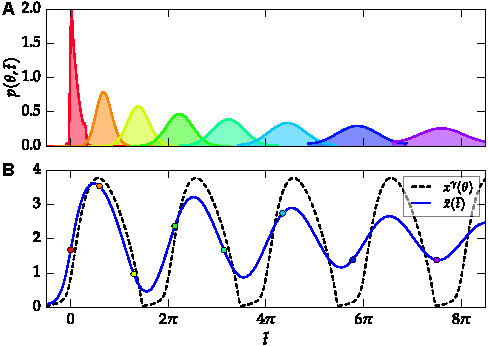
\includegraphics[width=.75\textwidth]{chap5/figures/figure_3.pdf}
  \titlecaption{Synchrony affects population-level amplitude}{ ({\bfseries A}) Stochastic fluctuations cause a population of cells to gradually desynchronize with time. The phase probability density, $p(\theta, \tilde{t})$, gradually widens as it advances in phase according to the mean period. ({\bfseries B}) The mean amplitude from a population of oscillators is determined by the probability density function $p(\theta, \tilde{t})$ and the oscillator's limit cycle $x^\gamma(\theta)$. As time passes, population-level rhythms resemble an exponentially damped sinusoid.}
  \label{fig:53}
\end{figure}

Next we describe how to calculate population-level mean expression following a perturbation.
The perturbed trajectory $\hat{x}(\tilde{t})$ can be decomposed into contributions from two sources.
First, for long times after the perturbation, each individual oscillator will have returned to the limit cycle $x^\gamma(\theta)$, but with a new population density $\hat{p}(\theta, \tilde{t})$.
This steady-state perturbed trajectory $\hat{x}_{ss}(\tilde{t})$ can be found by
\begin{equation}
  \hat{x}_{ss}(\tilde{t}) = \int_0^{2\pi} x^\gamma(\theta) \hat{p}(\theta, \tilde{t}) \; d\theta.
  \label{eq:xhatss}
\end{equation}
For very long times following perturbation, the new phase probability density could be approximated using the initial mean and standard deviation found through \fref{eq:zhat}, as jagged profiles in the population density will eventually smooth to a normal distribution.
However, for shorter times following perturbation, $\hat{p}(\theta, \tilde{t})$ must be calculated numerically.

The second contribution to the perturbed population trajectory comes from deviations from limit cycle oscillations in each cell.
We calculate the population-level effect of these deviations by averaging over the deviations that occur at each phase.
We define the deviation trajectory $\delta x(\theta, \tilde{t})$ for each phase as the distance between the perturbed trajectory and the phase-adjusted reference:
\begin{align}
  \delta x(\theta_0, \tilde{t}) &\coloneqq x(\tilde{t}) - x^\gamma(\tilde{t} + \theta_0 + \Delta \theta) \\
  \therefore\; \lim_{\tilde{t} \to \infty} \delta x(\theta, \tilde{t}) &= 0.
  \label{eq:deviation}
\end{align}
Since the perturbed trajectory ultimately converges with the phase-adjusted reference, deviations will converge to zero.
Since the phase change, $\Delta\theta$, associated with a perturbation at each phase is likely not known prior to calculating the perturbed trajectory, it is difficult to tabulate deviation trajectories associated with each final phase, $\theta_0 + \Delta\theta$.
It is therefore more straightforward to find the average effect of single-cell perturbations at the population level by weighting the deviations by the phase density function prior to perturbation.
The population-level response to a perturbation, $\hat{x}(\tilde{t})$, is therefore defined as
\begin{equation}
  \hat{x}(\tilde{t}) = \int_0^{2\pi} x^\gamma(\theta)\hat{p}(\theta, \tilde{t}) + \delta x(\theta, \tilde{t})p(\theta, \tilde{t}) \; d\theta.
  \label{eq:xhat}
\end{equation}
Here the first term is equivalent to $\hat{x}_{ss}(\tilde{t})$, the steady-state perturbed trajectory, while the second term decays to zero as individual oscillators return to their steady-state amplitude.
The accuracy of the continuous phase-diffusion model was tested by explicitly simulating a perturbation to a population of 225 uncoupled oscillators using a stochastic simulation algorithm \cite{Gillespie1977, Sanft2011a}.
Good agreement between the stochastic population and continuous approximation was shown in phase shift, single-cell level amplitude change, and alteration of population synchrony (\fref{fig:5s2}).
These results indicate the use of a continuous probability function is justified in the case of cultured cellular reporter systems, which may contain up to $10^5$ individual cells per culture \cite{Welsh2004}.
In addition, the method was verified by similar simulations using the Oregonator \cite{Field1974}, a model containing only mass-action terms, and a detailed mechanistic model of circadian rhythms \cite{Hirota2012} at a variety of phase timings (\fref{fig:5s3a} and \fref{fig:5s3b}).
Good agreement is seen between the continuous and stochastic simulations, indicating the proposed method is suitable for predicting the population-level responses for a variety of model types. 
The slightly reduced accuracy seen in the larger \fref{mod:hirota} demonstrates a limitation of the method, which should be considered before applying the method to extreme cases. 
As \fref{eq:deviation} tabulates the response of the system from the limit cycle, systems which are perturbed from states far from the deterministic limit cycle will not be captured appropriately. 
Therefore, the difference in accuracy between \fref{mod:hirota} and \fref{mod:oregon} likely comes from increased deviation about the deterministic limit cycle in a greater number of spatial dimensions. 
The continuous approximation is therefore able to capture the population-level dynamics of a wide variety of limit cycle models and perturbations.

\begin{figure}[tbp]
  \centering
  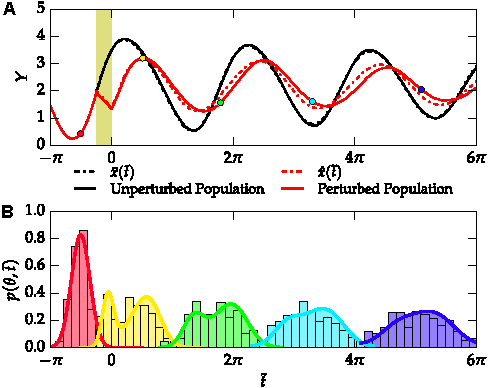
\includegraphics[width=.75\textwidth]{chap5/figures/figure_S2.pdf}
  \titlecaption{Approximation of an explicit stochastic population by continuous methods}{({\bfseries A}) A population of 225 stochastic oscillators was simulated using the Gillespie stochastic simulation algorithm (SSA). The mean protein expression, $Y$, is plotted as a function of time. A $50\%$ reduction in the protein translation rate to each of the oscillators is applied from $\hat{t} = -\nicefrac{\pi}{4} \to 0$, resulting in both single-cell and population-level amplitude change (red solid line). This population is approximated by the continuous methods described in this manuscript, in which the decay parameter $d=0.025$ is estimated to match the stochastic-induced desynchrony of the control population (black solid line). The initial standard deviation $\sigma_0 = 0.48$ is similarly matched to the stochastic population. The resulting predicted unperturbed and perturbed trajectories, $\bar{x}(\hat{t})$ and $\hat{x}(\hat{t})$ respectively, closely match the stochastically modeled values.  ({\bfseries B}) Phase histograms for the stochastic population are shown at several phases, both before and after the desynchronizing perturbation.  Phase probability-density functions for the continuous approximation are also shown, with close agreement between stochastic and continuous simulations. This close approximation validates the use of ODE models and phase-diffusion populations in deriving amplitude and phase-response behavior for networks of uncoupled cells.}
  \label{fig:5s2}
\end{figure}

\begin{figure}[tbp]
  \centering
  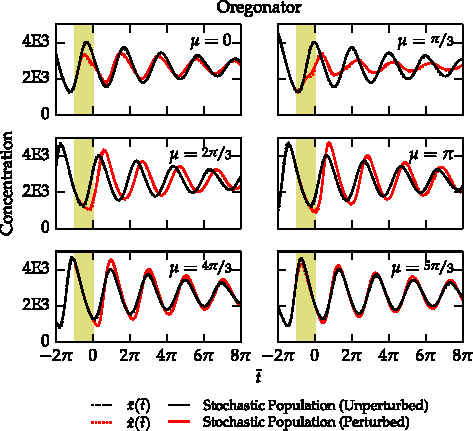
\includegraphics[width=0.75\textwidth]{chap5/figures/figure_S3a.pdf}
  \titlecaption{Validation of continuous methods with the Oregonator model}{ ({\bfseries A}) The Oregonator model (\fref{mod:oregon}) was tested as an example of a mass-action limit cycle oscillator. A population of 2000 oscillators was perturbed at size different mean phases, $\mu$, by increasing the $\mathit{c2}$ parameter by $50\%$ for $d=\pi$ (highlighted region). Only the average $\mathit{Y2}$ variable is plotted.}
  \label{fig:5s3a}
\end{figure}

\begin{figure}[tbp]
  \centering
  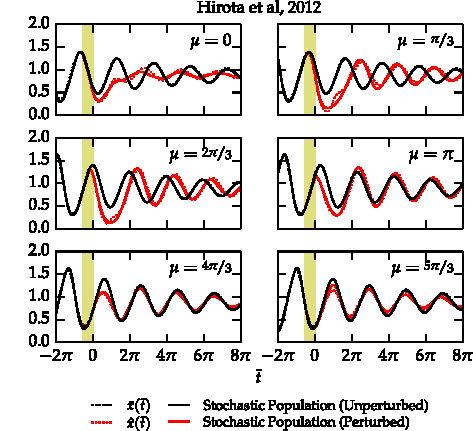
\includegraphics[width=0.75\textwidth]{chap5/figures/figure_S3b.pdf}
  \titlecaption{Validation of continuous methods with the model from Hirota {\itshape et al.,} 2012}{ ({\bfseries A}) ({\bfseries B}) The model described in \cite{Hirota2012} (\fref{mod:hirota}) was similarly tested at a variety of mean phases by reducing the $\mathit{vdp}$ parameter by $28.5\%$ and plotting the resulting $\mathit{c2}$ state variable (as in \fref{fig:55}). Parameters for the continuous approximations were found by estimating the phase, initial standard deviation, period, and phase diffusivity of the control population. }
  \label{fig:5s3b}
\end{figure}


\begin{model}[p]
  \titlecaption{The Oregonator model \cite{Field1974}}{The parameters used are as presented in \cite{Gillespie1977}. Used in \fref{fig:5s3a} as an example of a limit cycle oscillator using only mass-action kinetics.}
  \label{mod:oregon}

  The individual chemical reactions (used for stochastic simulation) are:
\begin{align*}
  X_1 + Y_2 &\xrightarrow{c_1} Y_1\\
  Y_1 + Y_2 &\xrightarrow{c_2} Z_1\\
  X_2 + Y_1 &\xrightarrow{c_3} 2Y_1 + Y_3\\
  2Y_1 &\xrightarrow{c_4} Z_2\\
  X_3 + Y_3 &\xrightarrow{c_5} Y_2
\end{align*}

These reactions can be converted to a standard ODE model, in which only the
intermediate variables $Y$ are considered, as:
\begin{align*}
  \frac{d\,\mathit{Y1}}{dt} &= \mathit{c1x1}\cdot\mathit{Y2} -
  \mathit{c2}\cdot\mathit{Y1}\cdot\mathit{Y2} + \mathit{c3x2}\cdot\mathit{Y1} -
  \mathit{c4}\cdot\mathit{Y1}^2\\
  \frac{d\,\mathit{Y2}}{dt} &= -\mathit{c1x1}\cdot\mathit{Y2} -
  \mathit{c2}\cdot\mathit{Y1}\cdot\mathit{Y2} + \mathit{c5x3}\cdot\mathit{Y3}\\
  \frac{d\,\mathit{Y3}}{dt} &= \mathit{c3x2}\cdot\mathit{Y1} -
  \mathit{c5x3}\cdot\mathit{Y3}
\end{align*}
  
\begin{center}
  \tablehead{\toprule Parameter & Value\\\midrule}
  \begin{supertabular}{rl}
    $\mathit{c1x1}$ & 2 \\
    $\mathit{c2}$ & 0.1 \\
    $\mathit{c3x2}$ & 104 \\
    $\mathit{c4}$ & 0.016 \\
    $\mathit{c5x3}$ & 26 \\
    \bottomrule\end{supertabular}
\end{center}
\end{model}

We next demonstrate the usefulness of single-cell and population level ARCs in predicting the mean response of a population.
Using a detailed single-cell model (\fref{mod:hirota}), we calculate the response of the system, specifically the average CRY2 protein expression level, to a temporary increase in {\itshape Per} transcription rate.
In part A of \fref{fig:54}, we plot the resulting single-cell and population-level response curves.
In this case, the population-level phase change is a slightly smoothed version of the single-cell PRC, since the population has an averaging effect on incoming perturbations with each cell receiving the input at a slightly different internal phase.
This smoothing follows from the consistent definition of phase between the single-cell and population level.
In the ARC plot, however, the shape of the single-cell and population-based ARC are different, since they describe different types of changes (finite vs.\ sustained) in the output trajectories.

\begin{figure}[tbp]
  \centering
  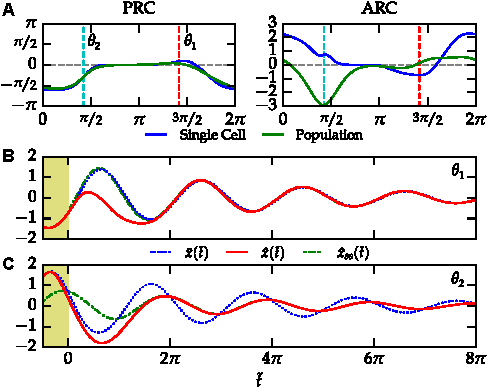
\includegraphics[width=.75\textwidth]{chap5/figures/figure_4.pdf}
  \titlecaption{Response curves describe different types of amplitude change}{A population of cells is simulated using a detailed model of circadian rhythms (\fref{mod:hirota}). Each cell in the population is subjected to a $20\%$ increase in the $\mathit{vtp}$ parameter ({\itshape Per} transcription rate) for $d=\nicefrac{\pi}{2}$, inducing both a phase and amplitude change. ({\bfseries A}) The phase response curves are shown for both the single limit cycle oscillator and population average, left. The population-level ARC is shown together with the single-cell amplitude response, with both curves normalized to $\sigma=1$. ({\bfseries B-C}) Population-level rhythms, $\hat{x}(\tilde{t})$ resulting from perturbations given at the indicated phases in A (red and cyan lines, respectively). The population transitions from the unperturbed population, $\bar{x}(\tilde{t})$, to the steady-state perturbed population, $\hat{x}_{ss}(\tilde{t})$. ({\bfseries B}) A perturbation at this phase yields a transient amplitude reduction resulting from perturbations at the single-cell level, however, there is little change in population synchrony. Population-level rhythms are therefore transiently damped before regaining normal amplitudes. ({\bfseries C}) Oscillators are desynchronized, but with a transient increase in limit cycle amplitude. It therefore takes some time before the amplitude reduction from desynchrony is realized.}
  \label{fig:54}
\end{figure}

Using these response curves, we demonstrate characteristic features of amplitude change mediated at the single-cell and population-level.
In part B of \fref{fig:54}, the perturbation at $\theta_1$ does not cause a significant change in phase or population synchrony, yet strongly reduces single-cell amplitudes.
The resulting population-level trajectory appears damped for the first cycle, until the oscillators within the population return to the limit cycle and normal amplitudes are restored.
In part C, the perturbation at $\theta_2$ reduces population synchrony while increasing single-cell amplitudes, yielding amplitudes that are transiently increased before the population settles to a lower-amplitude, desynchronized trajectory.

These examples demonstrate the qualitative differences between amplitude change mediated at the single-cell and population level.
Their characteristic features allow us to distinguish between these two sources of amplitude change without explicitly recording single-cell amplitudes: amplitude change induced at the population-level will be sustained, but may be masked in the short term by changes to single-cell level amplitudes.
Similarly, a change induced at the single-cell level will be evident only at short time-scales.
These results underscore the importance in considering both single-cell and population-mediated amplitude change in predicting the effects of daily stimuli on clock amplitudes.


\subsection{Application to Experimental Data}

We conclude by using the proposed modeling framework to reconcile two experimental studies that measured the effect of light on the circadian amplitude of photosensitive fibroblast cells \cite{Ukai2007, Pulivarthy2007}.
Both studies sought to determine the main factor of amplitude reduction following a transient light pulse, in which either desynchrony alone \cite{Ukai2007} or a combination of single-cell amplitude reduction and desynchrony \cite{Pulivarthy2007} was identified as the dominant factor.

Data on the response of melanopsin-responsive and control NIH3T3 mouse fibroblasts cells is shown in \fref{fig:55} \cite{Ukai2007}.
The experimental data is de-noised using a discrete wavelet transform \cite{Leise2011}.
In the experiment, a light pulse is given to desynchronize a colony of cells, resulting in drastically reduced amplitudes.
A second (longer) light pulse subsequently re-synchronizes the population, resulting in increased amplitudes.
To capture this phenomenon {\itshape in silico}, we used a recent model of the core circadian feedback circuit \cite{Hirota2012}.
In order to find parameters for the phase density function, we assumed an initial phase population with $\sigma = 0.1$ and calculated a phase diffusivity parameter $d = 0.104$ from the experimental control trajectory.

\begin{figure}[tbp]
  \centering
    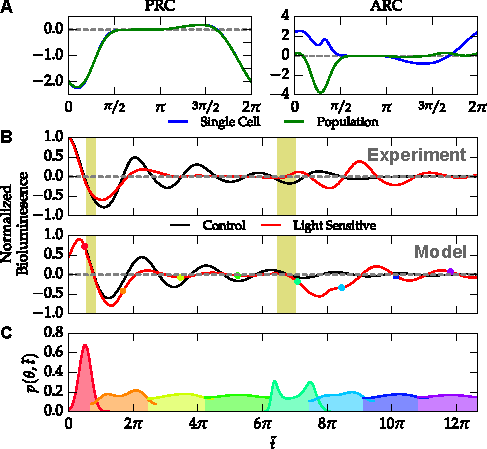
\includegraphics[width=.75\textwidth]{chap5/figures/figure_5.pdf}
    \titlecaption{Method allows direct comparison between model results and experimental bioluminescence profiles}{({\bfseries A}) Response curves for the parameter perturbation used to model the first light pulse in (B). The initial phase of the system is chosen to coincide with the strong dip in the population-level ARC (left). ({\bfseries B}) De-noised bioluminescence data from Ukai {\itshape et al.} 2007 (top) demonstrates population-level amplitude change resulting from two light pulses \cite{Ukai2007}. Circadian oscillations are suppressed by the first light pulse and rescued by the second. These perturbations were reproduced {\itshape in silico} (bottom) using the model from Hirota {\itshape et al.} 2012. The experimental results are qualitatively captured by the model, demonstrating the suitability of the method in capturing bioluminescence experiments. The relative amplitude of the model equations has been scaled to match that of the normalized bioluminescence profiles. ({\bfseries C}) Example probability density functions for the model trajectory shown in (A). The initial population (red) is effectively desynchronized (orange) following the first light pulse.}
    \label{fig:55}
\end{figure}

The next step in capturing the experimental data was finding a perturbation capable of desynchronizing the system.
To find such a perturbation, we calculated population-level ARCs at several different knockdown strengths for each parameter in the model.
We selected the degradation rate of {\itshape Per} mRNA from the feasible parameters due to PER's known induction by CREB following photo-perturbation \cite{Tischkau2003}.
While not an exact match of the experimental system, reducing degradation rate yields a similar response to increasing transcription.
The parameter was reduced by $28.5\%$ during the light pulses, a value fit to maximize light-induced desynchrony.
The output variable, PER2-luciferase in the experimental system, was chosen to be represented by {\itshape Cry1} mRNA - an E box activated gene that is buffered from the direct effects of the parameter perturbation.
The single-cell and population-level response curves for this parameter choice are shown in \fref{fig:55}, which demonstrates the strong desynchronization that occurs at $\theta\approx\nicefrac{\pi}{4}$.
Since the reporter used in the experimental system likely has a phase lag from the corresponding mRNA, we did not try to match the initial phase of the simulation to experiment.
Instead, the initial phase of simulation was chosen such that the first pulse occurred when the system was at the phase that corresponded with the minimum of the population-level ARC.

Population-level trajectories were found by solving for the resulting limit cycle trajectories at every phase, and subsequently finding the weighted average of these trajectories according the phase density (as described in equations~(\ref{eq:xbar} and \ref{eq:xhat})).
The simulated control and perturbed trajectories, Fig.~5B, closely match the experimental results, in which the model captures both the phase shifts and amplitude modulation of the light pulses.
The phase probability density function for the light-sensitive model trajectory is shown in Fig.~5C for several representative time points.
Changes to the synchronization of the population from each perturbation are readily apparent, with both perturbations inducing a bimodal distribution in the phase density.
While experimental data on individual cell phases was unavailable for this data set, bimodal distributions in SCN neuron firing following a phase shift have previously been seen experimentally \cite{Rohling2011}.
As higher-frequency features, these bimodal distributions dissipate as the phases diffuse.
Amplitude change in this case is mediated both at the population and single-cell level, as indicated by their representative ARCs. The contributions from each source are summarized in Fig.~S4.

Several quantitative differences between the model and experiment do appear.
Most importantly, the acute amplitude change following the light pulse is not correctly captured by the single-cell model.
From the experimental system, it appears the light pulse temporarily reduces PER2-luciferase amplitudes immediately following perturbation, separate from the overall change in population synchrony.
This result is most obvious after the second light pulse, where rhythms require some time before their maximum amplitude is reached.
Such a delay is indicative of perturbations to the limit cycle system, suggesting a contribution from single-cells in determining the population amplitude.
Light-induced amplitude suppression in fibroblasts is therefore likely mediated at the single-cell level at short time-scales, and at the population level for longer time-scales.
To improve the fit of the model to the data, the response curves could be fit to match experimentally predicted values.
Infinitesimal PRCs and ARCs calculated at the single-cell level are numerically efficient to evaluate, and could be more readily incorporated into a parameter estimation algorithm than explicit stochastic simulations of a population of oscillators.

\section{Conclusion}

In this chapter, we have described new tools for understanding amplitude change in independent cells based on analytically tractable methods for simulating a large population of oscillators.
These tools synthesize single-cell level ODE sensitivity analysis metrics with population-level measures of synchrony, allowing the quantification of clock amplitude at multiple levels of biological organization.
Using these tools, we have demonstrated how ODE models can be directly compared to experimental bioluminescence profiles, which currently serve as a standard system to investigate clock perturbations.
More generally, we have demonstrated the differences between acute and prolonged changes in amplitude following temporary perturbations, and characterized the mechanisms that give rise to each.

\subsection{Application to pharmacological control}
While our examples have focused on light-mediated perturbations, these approaches could also be applied to pharmacological perturbations.
Some difficulty arises in obtaining such data in cultured cells, however, as entraining perturbations would require that pharmacological agents be introduced for only a finite duration.
As medium or temperature changes are often enough to resynchronize cultured cells, a transient application is difficult to achieve experimentally.
The search for clock-enhancing molecules has therefore tended to focus on constant drug concentrations: for instance, dose-dependent period or amplitude change following inhibition of CK1$\delta$ or similar targets \cite{Chen2013}.
For {\itshape in vivo} systems, however, pharmacokinetics dictates a finite duration of action for both naturally secreted hormones and pharmacological therapies.
More effective treatments might therefore be designed by explicitly accounting for such a transient response, perturbing peripheral clocks at the right phase to induce resynchronization and an increase in single-cell level amplitudes.

Maintaining robust rhythmicity in peripheral oscillators has been linked to protection against metabolic disease.
It is therefore interesting that liver cells have not developed a stronger mechanism of intercellular coupling, such as in the SCN, to maintain robust amplitudes in the absence of external cues.
Perhaps the ability to quickly re-entrain to a phase shift, which is often slowed by coupling \cite{Abraham2010}, has historically been more advantageous than protection against highly variable food intake.
Regardless, the necessities of modern society often dictate irregular circadian-metabolic regimes that damp peripheral clock oscillations.
For such instances, we hope that the mathematical theory presented here will permit the development of optimized treatment regimes.

\subsection{Damping rate is correlated with single-cell noise}

One result from this chapter, which has previously been discussed in the circadian literature \cite{Rougemont2007}, is that in noninteracting populations, stochastic noise at the single-cell level affects the damping rate of a population of oscillators. 
Stochastic noise is often a relevant circadian parameter, as it describes the precision of the underlying oscillators. 
In the following chapter, I show how population-level recordings, even those from high-throughput circadian screens, can be used to gain estimates of stochastic noise at the single-cell level. 
Using such an approach, it is possible to gain genome-wide insight into how noise is regulated in the cell-autonomous feedback loop. 
